% Generated by tools/build_paper_tables.py from robustness.json.
The strengthened family-wide intervals change the interpretation of the local result (Fig.~\ref{fig:overview}A). All 12 peer intervals include zero. For Qwen3 P02 at 11:00, the simultaneous interval is [-17.7, 59.5] pp, substantially wider than its pointwise interval. This conservative result does not prove no effect; it shows that the present data and family-wide criterion do not support a positive conclusion selected from all 12 contrasts.

Batch resampling gives a pointwise interval of [11.1, 43.9] pp for the same profile. It retains a positive local response under this grouping sensitivity, while neither addressing multiplicity nor expanding the target to human students. All 10,000 resamples for every contrast were defined. At zero-success boundaries several bootstrap intervals collapse to [0, 0]; these are empirical-support artifacts, not substitutes for binomial uncertainty.

\begin{figure*}[t]
\centering
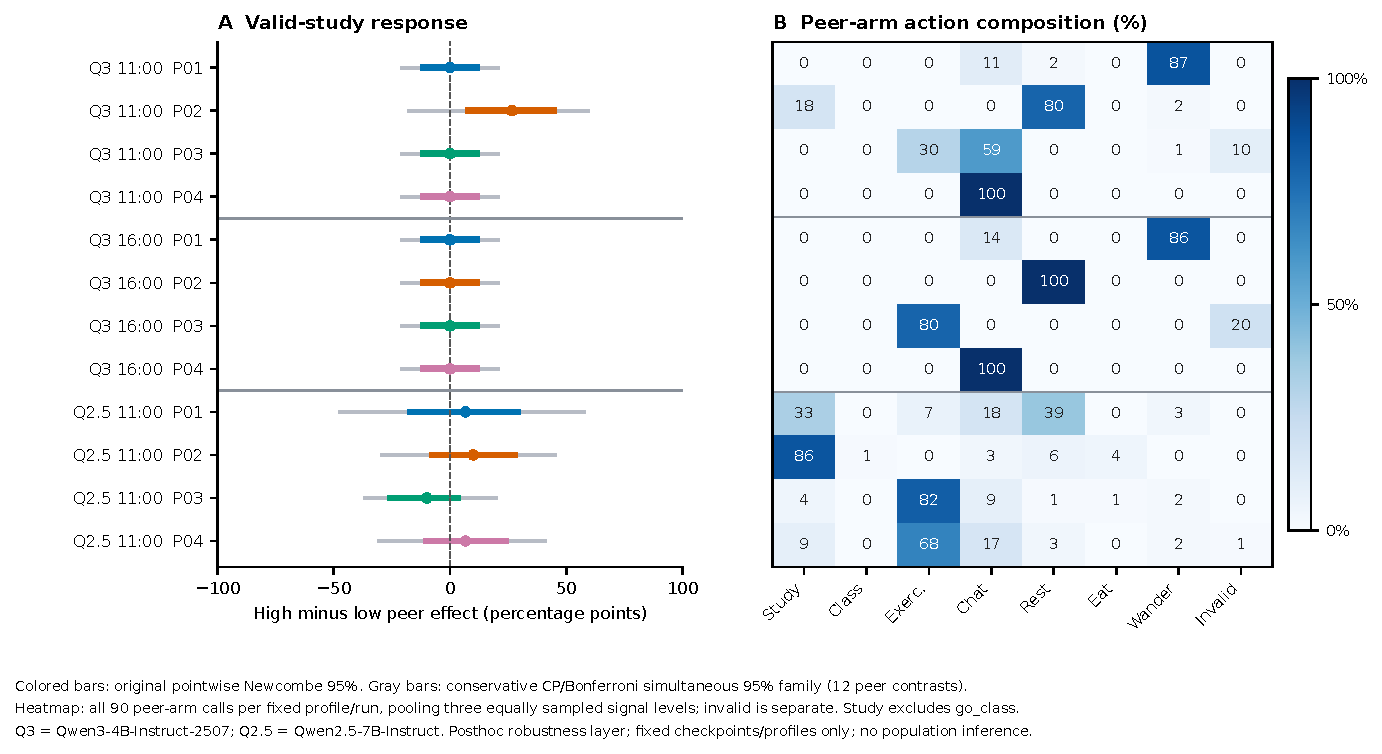
\includegraphics[width=\textwidth]{figures/robustness_overview.pdf}
\caption{Peer-response audit. (A) High-minus-low valid-study differences: colored bars are original pointwise Newcombe 95\% intervals; gray bars are conservative Clopper--Pearson/Bonferroni intervals with at least 95\% simultaneous coverage for the complete 12-contrast peer family under the stated assumptions. (B) Seven valid actions plus invalid outputs, pooling the three equally sampled peer levels (90 completed calls per profile/run). Pooling describes baseline composition; it is not the peer-effect estimator. Q3 and Q2.5 denote the two fixed checkpoints.}
\label{fig:overview}
\end{figure*}
